
%\newpage
\section{Measurement of frequency}
\label{sec:frequency}

Beginning with Version 1.10k the frequency measurement can be selected with a control menu.
The normal frequency measurement is done with counting the falling edges of input signal T0 (PD4)
with counter 0 für one second. For maintaining of a accurate second, the counter 1 is used
with a 256:1 prescaler of the CPU frequency. 
The 16 bit counter of the ATmega can be used up to 16 MHz CPU frequency with the prescaler to
serve the second period in one pass.
For the start and stop of the counter 0 ist the compare register B and A of the counter 1 used.
To prevent a unstable delay by polling the compare event signals, for starting and stopping the
Interrupt Service of both counter 1 compare events is used.
The time delay of both Interrupt Service Routines is nearly equal.
To maintain a accurate second period is a constant delay insignificant.
With analysing the assembler code, the difference in time can be adjusted.\\

For frequencies below \(25 kHz\) the normal measurement is followed by a measurement of
period time. This additional measurement is only followed after a normal frequency measurement.
This will be done by measuring the time of a selectable count of the Pin Change interrupts
of the PCINT20 (PD4) input with the counter 0.
By measuring the period both, the negative puls width and the positive puls width, should be
at least \(10\mu s\) .
The counter 0 is used with full clock rate. This results to a resolution of \(125 ns\) for
\(8 MHz\). With a greater count of measurements periods the resolution can be reduced.
By using a measurement period of 125 periods, the middle resolution for one period is \(1 ns\).
To prevent the inexactness of start and stop the counter 0, the start of counter 0 is started
within the first pin change interrupt of PCINT20 and will be stopped with the last pin change interrupt
with the same interrupt service routine.
The count of periodes is choosed, that the measurement time is about 10 million clock tics.
The part of error from one clock is only 0.1ppm with this choise.
With a \(8 MHz\) clock the measurement time is about 1.25 seconds.
From this mean value of one period a frequency with better resolution is computed too.

For checking the procedure, two testers are measured against each other.
First the test frequencies are generated with tester 2 and measured with tester 1.
After that the testers are swapped and the measurement is repeated.
Figure \ref{fig:freq-ppm} shows the results of both measurement series.
The nearly constant errors can be explained with a little frequency difference of both crystals.

\begin{figure}[H]
\centering
% GNUPLOT: LaTeX picture with Postscript
\begingroup
  \makeatletter
  \providecommand\color[2][]{%
    \GenericError{(gnuplot) \space\space\space\@spaces}{%
      Package color not loaded in conjunction with
      terminal option `colourtext'%
    }{See the gnuplot documentation for explanation.%
    }{Either use 'blacktext' in gnuplot or load the package
      color.sty in LaTeX.}%
    \renewcommand\color[2][]{}%
  }%
  \providecommand\includegraphics[2][]{%
    \GenericError{(gnuplot) \space\space\space\@spaces}{%
      Package graphicx or graphics not loaded%
    }{See the gnuplot documentation for explanation.%
    }{The gnuplot epslatex terminal needs graphicx.sty or graphics.sty.}%
    \renewcommand\includegraphics[2][]{}%
  }%
  \providecommand\rotatebox[2]{#2}%
  \@ifundefined{ifGPcolor}{%
    \newif\ifGPcolor
    \GPcolortrue
  }{}%
  \@ifundefined{ifGPblacktext}{%
    \newif\ifGPblacktext
    \GPblacktexttrue
  }{}%
  % define a \g@addto@macro without @ in the name:
  \let\gplgaddtomacro\g@addto@macro
  % define empty templates for all commands taking text:
  \gdef\gplbacktext{}%
  \gdef\gplfronttext{}%
  \makeatother
  \ifGPblacktext
    % no textcolor at all
    \def\colorrgb#1{}%
    \def\colorgray#1{}%
  \else
    % gray or color?
    \ifGPcolor
      \def\colorrgb#1{\color[rgb]{#1}}%
      \def\colorgray#1{\color[gray]{#1}}%
      \expandafter\def\csname LTw\endcsname{\color{white}}%
      \expandafter\def\csname LTb\endcsname{\color{black}}%
      \expandafter\def\csname LTa\endcsname{\color{black}}%
      \expandafter\def\csname LT0\endcsname{\color[rgb]{1,0,0}}%
      \expandafter\def\csname LT1\endcsname{\color[rgb]{0,1,0}}%
      \expandafter\def\csname LT2\endcsname{\color[rgb]{0,0,1}}%
      \expandafter\def\csname LT3\endcsname{\color[rgb]{1,0,1}}%
      \expandafter\def\csname LT4\endcsname{\color[rgb]{0,1,1}}%
      \expandafter\def\csname LT5\endcsname{\color[rgb]{1,1,0}}%
      \expandafter\def\csname LT6\endcsname{\color[rgb]{0,0,0}}%
      \expandafter\def\csname LT7\endcsname{\color[rgb]{1,0.3,0}}%
      \expandafter\def\csname LT8\endcsname{\color[rgb]{0.5,0.5,0.5}}%
    \else
      % gray
      \def\colorrgb#1{\color{black}}%
      \def\colorgray#1{\color[gray]{#1}}%
      \expandafter\def\csname LTw\endcsname{\color{white}}%
      \expandafter\def\csname LTb\endcsname{\color{black}}%
      \expandafter\def\csname LTa\endcsname{\color{black}}%
      \expandafter\def\csname LT0\endcsname{\color{black}}%
      \expandafter\def\csname LT1\endcsname{\color{black}}%
      \expandafter\def\csname LT2\endcsname{\color{black}}%
      \expandafter\def\csname LT3\endcsname{\color{black}}%
      \expandafter\def\csname LT4\endcsname{\color{black}}%
      \expandafter\def\csname LT5\endcsname{\color{black}}%
      \expandafter\def\csname LT6\endcsname{\color{black}}%
      \expandafter\def\csname LT7\endcsname{\color{black}}%
      \expandafter\def\csname LT8\endcsname{\color{black}}%
    \fi
  \fi
  \setlength{\unitlength}{0.0500bp}%
  \begin{picture}(7200.00,5040.00)%
    \gplgaddtomacro\gplbacktext{%
      \csname LTb\endcsname%
      \put(814,704){\makebox(0,0)[r]{\strut{}-25}}%
      \csname LTb\endcsname%
      \put(814,1156){\makebox(0,0)[r]{\strut{}-20}}%
      \csname LTb\endcsname%
      \put(814,1609){\makebox(0,0)[r]{\strut{}-15}}%
      \csname LTb\endcsname%
      \put(814,2061){\makebox(0,0)[r]{\strut{}-10}}%
      \csname LTb\endcsname%
      \put(814,2513){\makebox(0,0)[r]{\strut{}-5}}%
      \csname LTb\endcsname%
      \put(814,2966){\makebox(0,0)[r]{\strut{} 0}}%
      \csname LTb\endcsname%
      \put(814,3418){\makebox(0,0)[r]{\strut{} 5}}%
      \csname LTb\endcsname%
      \put(814,3870){\makebox(0,0)[r]{\strut{} 10}}%
      \csname LTb\endcsname%
      \put(814,4323){\makebox(0,0)[r]{\strut{} 15}}%
      \csname LTb\endcsname%
      \put(814,4775){\makebox(0,0)[r]{\strut{} 20}}%
      \csname LTb\endcsname%
      \put(946,484){\makebox(0,0){\strut{} 1}}%
      \csname LTb\endcsname%
      \put(1783,484){\makebox(0,0){\strut{} 10}}%
      \csname LTb\endcsname%
      \put(2619,484){\makebox(0,0){\strut{} 100}}%
      \csname LTb\endcsname%
      \put(3456,484){\makebox(0,0){\strut{} 1000}}%
      \csname LTb\endcsname%
      \put(4293,484){\makebox(0,0){\strut{} 10000}}%
      \csname LTb\endcsname%
      \put(5130,484){\makebox(0,0){\strut{} 100000}}%
      \csname LTb\endcsname%
      \put(5966,484){\makebox(0,0){\strut{} 1e+06}}%
      \csname LTb\endcsname%
      \put(6803,484){\makebox(0,0){\strut{} 1e+07}}%
      \put(176,2739){\rotatebox{-270}{\makebox(0,0){\strut{}Error / ppm}}}%
      \put(3874,154){\makebox(0,0){\strut{}frequency / Hz}}%
    }%
    \gplgaddtomacro\gplfronttext{%
    }%
    \gplbacktext
    \put(0,0){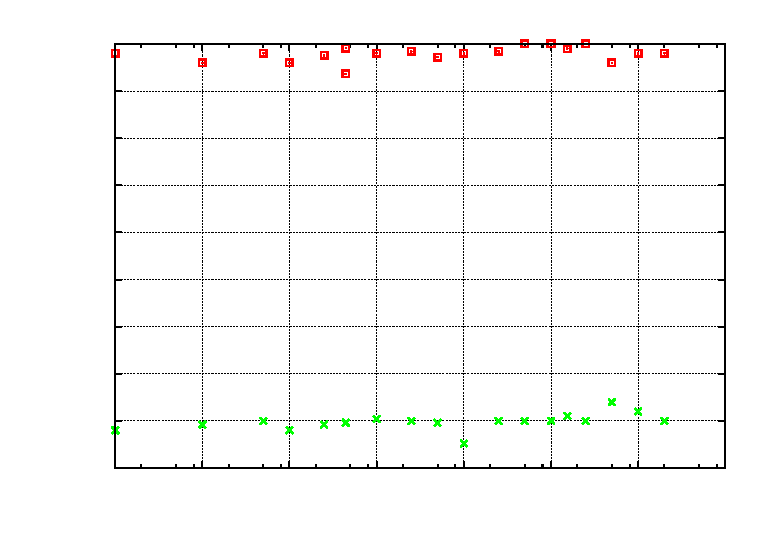
\includegraphics{../GNU/frequency-ppm}}%
    \gplfronttext
  \end{picture}%
\endgroup

\caption{Relativ erros of frequency measurement}
\label{fig:freq-ppm}
\end{figure}

Tuning of the cystal frequency is possible with a adjustable capacitor (5-25 pF) at the crystal.
The one pulse per second (1PPS) from the GPS receiver {\bf UP501} from {\bf Fastrax Ltd.} and from the GPS/GLONASS receiver
{\bf GNS701} from {\bf Global Navigation Systems GmbH} has been tested successfully for the calibration of the
crystal frequency.
The measured period could be adjusted to exactly \(1000.000 ms\).
Only the last digit can toggle with one unit.
Of course the frequency of the crystal is temperature dependent.
Therefore you can not expect a very good long time stability.

The figure \ref{fig:GPS-1PPS} shows the used circuits with a UM232 USB-serial converter
as connection of the receiver modules to a computer.
The UM232 converter support the circuit sowohl with both, the 5V and the 3.3V supply voltage
from the USB supply voltage.
No connection to a computer is required for operating the receivers.
Only the 5V supply voltage must be provided to the USB connector.

\begin{figure}[H]
  \begin{subfigure}[b]{9cm}
    \centering
    
\includegraphics[width=8.5cm]{../FIG/GPS_UP501.eps}
    \caption{GPS}
  \end{subfigure}
  ~
  \begin{subfigure}[b]{9cm}
    \centering
    
\includegraphics[width=8.5cm]{../FIG/GPS_GNS701.eps}
    \caption{GPS/GLONASS}
  \end{subfigure}
  \caption{Generation of a 1PPS signal with GPS receiver }
  \label{fig:GPS-1PPS}
\end{figure}
